\documentclass[preprint,12pt,nopreprintline]{elsarticle}
\usepackage{amssymb,amsmath,booktabs,url,hyperref,float,array,graphicx}
\journal{Geodata and AI}
\begin{document}
\begin{frontmatter}
\title{Supplementary Material for\\Tolerance-Aware Reservoir Property Prediction from Wireline Logs:\\Representation Complementarity, Decision Sensitivity, and Offline Transfer}
\author[aff1]{Minjie Chen\fnref{fn1}\corref{cor1}}
\ead{1269736732@qq.com}
\author[aff2]{Jiawei Xin\fnref{fn1}}
\author[aff1]{Chengfeng Wu}

\fntext[fn1]{These authors contributed equally to this work.}
\cortext[cor1]{Corresponding author.}

\affiliation[aff1]{organization={PetroChina Southwest Oil \& Gasfield Company},city={Chengdu},postcode={610051},country={China}}
\affiliation[aff2]{organization={China Telecom Corporation Limited Beijing Branch},city={Beijing},country={China}}
\end{frontmatter}
\clearpage
\renewcommand{\thefigure}{S\arabic{figure}}
\renewcommand{\thetable}{S\arabic{table}}

\section{S1. Public Volve benchmark extended details}
\label{sec:supp-public}
This section provides extended documentation for the public North Sea Volve/PDDA benchmark reproduction. The complete dataset comprises nine designated training boreholes and four released test boreholes. All models were trained strictly from scratch without utilizing internal industrial data or pre-trained parameter weights. Table~\ref{tab:public-metrics} documents the overall pooled RMSE alongside the auxiliary tolerance utility diagnostic across five distinct model variants. Table~\ref{tab:public-wells} breaks down the per-well RMSE across the four released test wells.

\begin{table}[t]
\centering
\caption{Public Volve reproducibility check. RMSE is pooled over VSH, PHIF and SW. Auxiliary tolerance is $\max(0,1-|a-y|/[c(|y|+10^{-7})])$, with $c=0.08$ for PHIF and $c=0.05$ for SW; it is not the contest's primary RMSE metric. Tolerance actions use 600 grid points between each target's bin representatives.}
\label{tab:public-metrics}
\small
\resizebox{\textwidth}{!}{%
\begin{tabular}{l ccccc}
\toprule
Variant & RMSE & PHIF RMSE & SW RMSE & PHIF tol. & SW tol. \\
\midrule
RF, five logs & 0.11082 & 0.02635 & 0.15773 & 0.33926 & 0.38002 \\
Tree regression & 0.10789 & 0.02443 & 0.16040 & 0.40916 & 0.26649 \\
Distribution, mean & 0.11847 & 0.02474 & 0.17629 & 0.48631 & 0.02209 \\
Distribution, tolerance action & 0.11480 & 0.02546 & 0.17195 & 0.51583 & 0.19359 \\
Tree regression + joint SW gate & 0.10619 & 0.02443 & 0.15696 & 0.40916 & 0.46368 \\
\bottomrule
\end{tabular}}
\end{table}

\begin{table}[t]
\centering
\caption{Per-well RMSE for the public baseline, target-specific regression and the joint SW gate. A pooled improvement need not occur in every well.}
\label{tab:public-wells}
\small
\setlength{\tabcolsep}{12pt}
\begin{tabular}{l cccc}
\toprule
Variant & Well 100 & Well 101 & Well 103 & Well 104 \\
\midrule
RF, five logs & 0.15282 & 0.10997 & 0.10013 & 0.06132 \\
Tree regression & 0.14917 & 0.12295 & 0.08280 & 0.04823 \\
Tree + joint SW gate & 0.14452 & 0.12334 & 0.08271 & 0.04783 \\
\bottomrule
\end{tabular}
\end{table}


\begin{figure}[H]
\centering
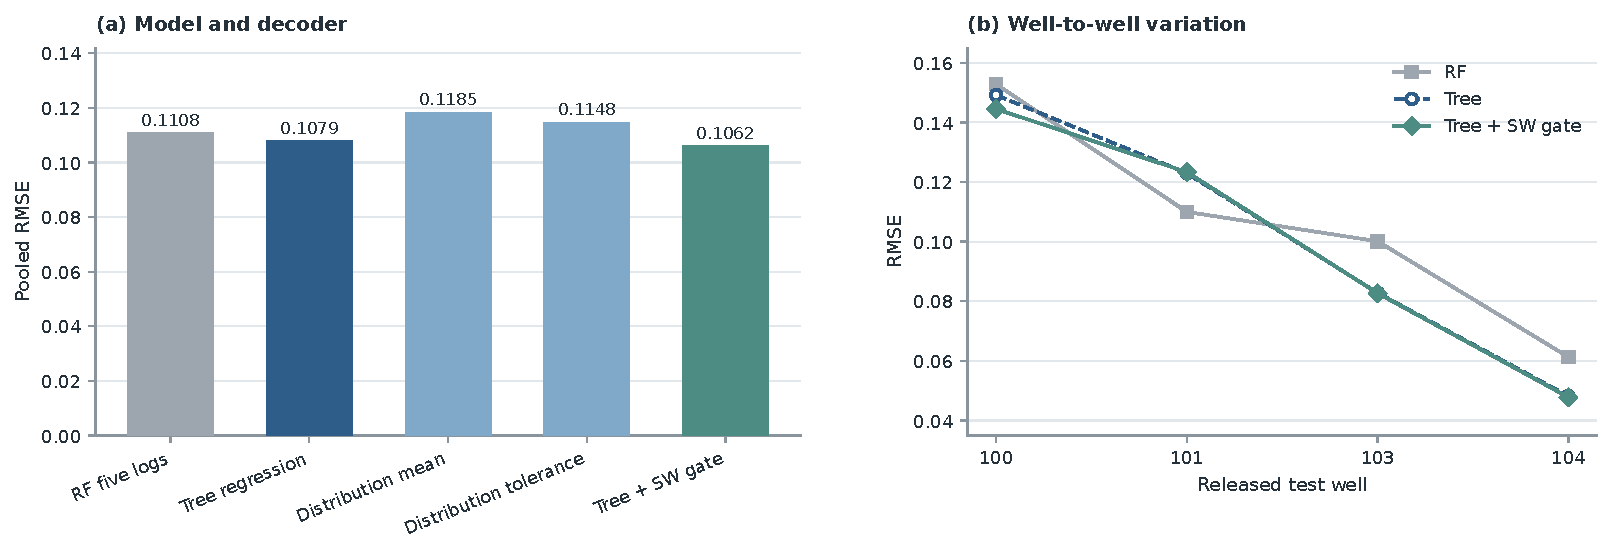
\includegraphics[width=\textwidth]{figures/fig_public_volve_paper.pdf}
\caption{Comprehensive public Volve performance comparison. (a) Pooled RMSE across models, where the tree model with a joint $\mathrm{SW}$ gate attains the lowest error (0.10619). (b) Disaggregated RMSE across the four released test wells, demonstrating inter-well geological variance.}
\label{fig:supp-public}
\end{figure}

For historical context, the leading published competition entries from the 2021 SPWLA PDDA benchmark \cite{fu2024contest} achieved pooled RMSEs of 0.0525 (UTFE, linear regression with extensive feature engineering), 0.0602 (MoLPhy, physics-guided ensemble), and 0.0634 (Tomsk, deep neural network), against the official PDDA random-forest reference of 0.11718 \cite{pddasig2021}. These published contest entries used different modelling pipelines, feature-engineering choices and development protocols. They provide context for task difficulty rather than a matched from-scratch comparison with our reproduction.

\section{S2. Detailed target breakdown of the public v4 boundary case}
\label{sec:supp-v4}
To establish the operational limits of architectural complexity, the complete v4 sequence pipeline was trained from scratch on the nine public training wells. The public network employs the three final heads (\texttt{por\_anchored}, \texttt{perm\_split}, and \texttt{sw\_density}) mapping to $\mathrm{PHIF}$, $\mathrm{SW}$, and $\mathrm{VSH}$, respectively. Checkpoints were selected independently across three folds based on validation loss.

\begin{table}[H]
\centering
\caption{Disaggregated target-level RMSE on the public Volve released test set.}
\label{tab:supp-v4-targets}
\small
\resizebox{\linewidth}{!}{%
\begin{tabular}{lcccc}
\toprule
Model configuration & Pooled RMSE & $\mathrm{PHIF}$ RMSE & $\mathrm{SW}$ RMSE & $\mathrm{VSH}$ RMSE \\
\midrule
Tree + joint $\mathrm{SW}$ gate & \textbf{0.10619} & \textbf{0.02443} & \textbf{0.15696} & \textbf{0.09270} \\
v4 root dual-backbone & 0.13794 & 0.03532 & 0.16660 & 0.16756 \\
Complete 18-stage v4 chain & 0.14695 & 0.03528 & 0.18806 & 0.16785 \\
v4 full chain (training OOF) & 0.09228 & 0.02415 & 0.12788 & 0.09278 \\
\bottomrule
\end{tabular}%
}
\end{table}

\begin{table}[H]
\centering
\caption{Borehole-by-borehole test RMSE comparison between the complete v4 sequence chain and the target-specific tree--gate baseline.}
\label{tab:supp-v4-wells}
\small
\begin{tabular}{lcc}
\toprule
Test borehole & Complete 18-stage v4 chain & Tree + joint $\mathrm{SW}$ gate \\
\midrule
Well 100 & 0.15879 & \textbf{0.14452} \\
Well 101 & 0.16418 & \textbf{0.12334} \\
Well 103 & 0.11580 & \textbf{0.08271} \\
Well 104 & 0.13965 & \textbf{0.04783} \\
\bottomrule
\end{tabular}
\end{table}

As documented in Table~\ref{tab:supp-v4-targets} and Table~\ref{tab:supp-v4-wells}, the complete 18-stage chain exhibits a substantial out-of-domain generalization gap: despite achieving a training OOF RMSE of 0.09228 on the nine training wells, its error increases to 0.14695 on the test wells. The tree--gate model maintains higher accuracy across all four individual test wells. The large training-to-test gap is consistent with overfitting under limited geological diversity, but does not by itself identify a unique causal mechanism.

\section{S3. Extended model-family development trajectory}
\label{sec:supp-trajectory}
Figure~\ref{fig:supp-model-family} visualizes the developmental progression across model generations (v1 through v4) on the internal industrial dataset. Connecting lines highlight the trajectory across configurations; however, because different developmental estimators were utilized across project milestones, these curves represent historical platform progression rather than a unified common-protocol ablation.

\begin{figure}[H]
\centering
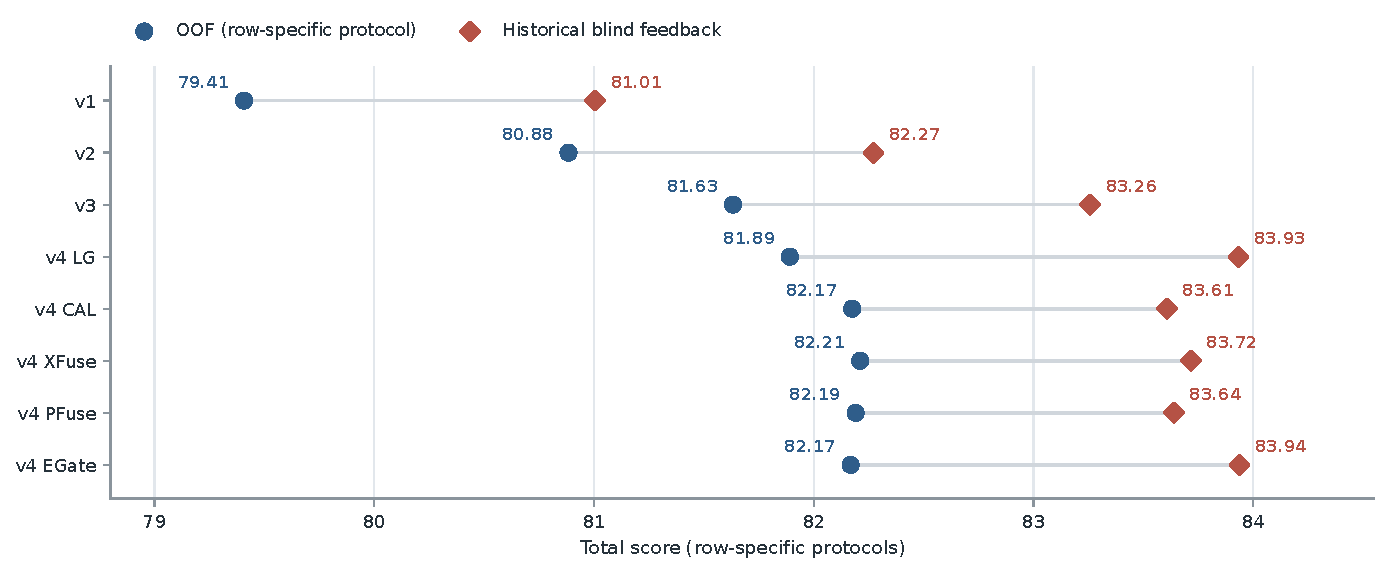
\includegraphics[width=\textwidth]{figures/fig_model_family_comparison.pdf}
\caption{Visual trajectory of internal model generations across five-fold cross-validation (OOF) and historical platform blind test submissions. Note that ranking inversions occur between OOF and blind scores.}
\label{fig:supp-model-family}
\end{figure}

\section{S4. Exploratory transfer and robustness diagnostics}
\label{sec:supp-exploratory}

\subsection{Type-well matching and dynamic time warping}
We evaluated whether spatial proximity or curve shape similarity could guide local transfer. Type-well matching via Dynamic Time Warping (DTW) on standardized gamma-ray and multi-log sequences was integrated into the fusion layer. Candidate neighbors were restricted strictly to permissible training folds. DTW-assisted fusion shifted the internal composite score from 81.6324 to 81.6421—a negligible increment (+0.01 points) within empirical bootstrap noise. Similarly, on the Volve benchmark, two-nearest-well training reduced $\mathrm{PHIF}$ RMSE slightly from 0.02137 to 0.01967, but severely inflated $\mathrm{SW}$ RMSE from 0.08828 to 0.16501. Consequently, DTW alignment does not provide a universal transfer mechanism.

\subsection{Distribution drift and Kolmogorov--Smirnov analysis}
To investigate whether blind-well performance drops were driven by anomalous input curve drift, we computed the two-sample Kolmogorov--Smirnov (KS) statistic for each logging channel across the ten blind wells relative to the training population. Figure~\ref{fig:supp-drift} displays the resulting mean KS distances plotted against the empirical leave-one-well-out reference range of the training set.

\begin{figure}[H]
\centering
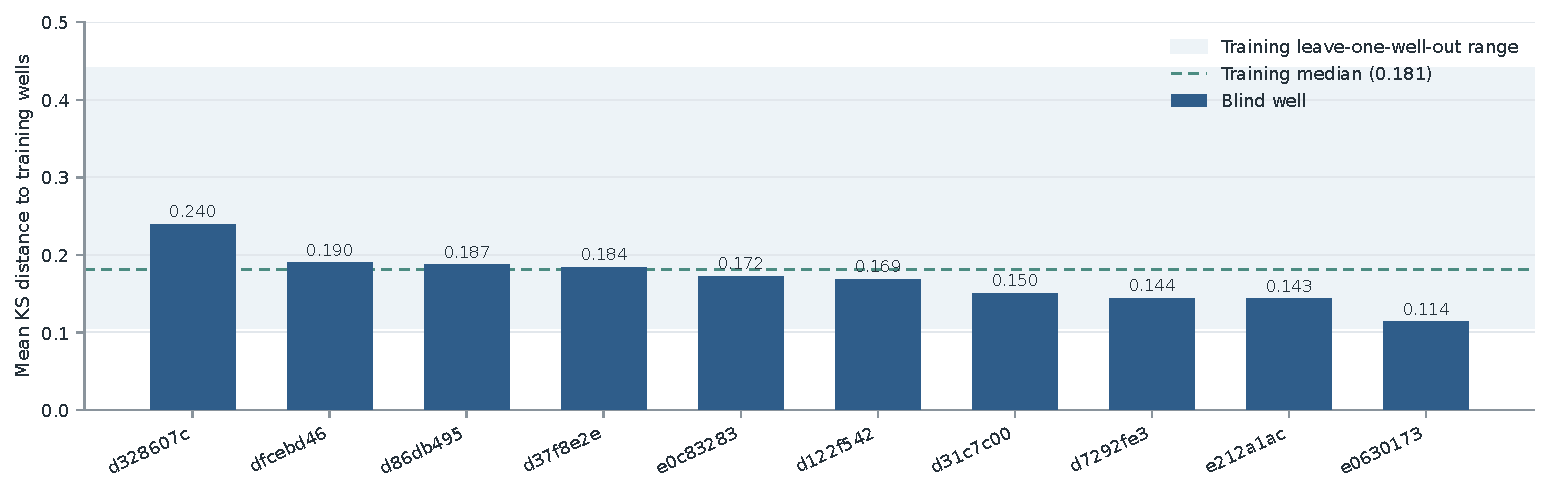
\includegraphics[width=\textwidth]{figures/fig9_drift_profile.pdf}
\caption{Mean Kolmogorov--Smirnov (KS) drift profile of the ten blind test wells relative to the training population, benchmarked against the leave-one-well-out baseline reference range.}
\label{fig:supp-drift}
\end{figure}

All blind-well mean KS values fall within the empirical training distribution range. This diagnostic does not support anomalous measured input drift as the primary explanation, but it does not exclude label shift, local calibration differences or shifts outside the measured statistics.

\subsection{Synthetic sensor perturbation probe}
To test sequence network robustness against logging tool miscalibration, we conducted synthetic gain/offset perturbation probes. Random gain ($\pm 10\%$) and offset ($\pm 5\%$) perturbations were applied to logging curves. When trained without augmentation, the $\mathrm{SW}$ head suffered a substantial performance drop of $-0.694$ utility points. Applying stochastic gain/offset augmentation during training reduced this decrement to $-0.033$ points, while the clean evaluation score remained virtually unchanged (74.844 vs. 74.739). This synthetic probe shows improved robustness under the tested perturbations; it is not evidence of improved hidden-well accuracy or field-wide instrument invariance.

\section{S5. Evidence protocols and uncertainty quantification}
\label{sec:supp-protocols}
A rigorous distinction must be maintained between different sources of empirical uncertainty:
\begin{enumerate}
\item \textbf{Spatial well-bootstrap confidence intervals}: The paired bootstrap intervals ($B=1,000$ resamples) reported in the main text resample entire boreholes with replacement. These intervals quantify spatial sampling variability conditional on the fitted model weights.
\item \textbf{Random seed handling}: In the retrained $\mathrm{PERM}$ bin-count experiments ($K \in \{30, 60, 120\}$), each configuration uses the same two fixed seeds, five-fold splits and 1,200 boosting iterations, and is evaluated as a two-seed ensemble. Legacy fusion OOF arrays were already seed-averaged, so separate seed-wise ablation variance is not identifiable from those arrays.
\item \textbf{Post-hoc sensitivity sweeps}: Parameter sweeps across continuous mixing weights, gate decision thresholds, and bin counts evaluate local landscape geometry and robustness; they do not construct new independent blind tests.
\end{enumerate}
Together, spatial well-bootstrap confidence bounds and multi-seed evaluations establish a rigorous statistical basis for model selection and performance consistency across variable geological strata.

\bibliographystyle{elsarticle-num}
\bibliography{refs}
\end{document}
